
\documentclass[aspectratio=169]{beamer}
\usetheme{metropolis}           % Use metropolis theme
\usepackage[utf8]{inputenc}
\usepackage{graphicx}
\usepackage{eso-pic}
\usepackage{graphics}
\usepackage{tikz}
\usepackage[export]{adjustbox}
\usepackage{multicol}
\usepackage{listings}
\usepackage{helvet}
\usepackage{booktabs}
\usepackage{threeparttable}


\title{Introduction to Stata}
\date{\today}
\author{Author of Session here!} % Name of author(s) of session here
\institute{Development Impact Evaluation (DIME) \newline The World Bank }
\setbeamercolor{background canvas}{bg=white}	% Sets background color

% The below command places the World Bank logo and DIME logo to the right corner
\titlegraphic{%
	\begin{picture}(0,0)
	\put(330,-180){\makebox(0,0)[rt]{
\includegraphics[width=3cm]{img/WB_logo}}}
	\end{picture}%
	\begin{picture}(0,0)
	\put(390,-180){\makebox(0,0)[rt]{
\includegraphics[width=1.5cm]{img/i2i}}}
	\end{picture}%
}

%%% Section page with picture of Light bulb
\makeatletter
\defbeamertemplate*{section page}{mytheme}[1][]{
	\centering
	\begin{minipage}{22em}
		\raggedright
		\usebeamercolor[fg]{section title}
		\usebeamerfont{section title}
		\par
		\ifx\insertsubsectionhead\@empty\else%
		\usebeamercolor[fg]{subsection title}%
		\usebeamerfont{subsection title}%
		\fi
		\ifstrempty{#1}{}{%
			\includegraphics[width=100mm, height=60mm]{#1}%
		}
		\insertsectionhead\\[-1ex]
		\insertsubsectionhead
		\usebeamertemplate*{progress bar in section page}
		
	\end{minipage}
	\par
	\vspace{\baselineskip}
}
\makeatother

%%% Define a command to include picture in section, 
%%% make section, and revert to old template
\newcommand{\sectionpic}[2]{
	\setbeamertemplate{section page}[mytheme][#2]
	\section{#1}
	\setbeamertemplate{section page}[mytheme]
}

%%% The command below allows for the text that contains Stata code
\lstset{ %
	backgroundcolor=\color{white},
	basicstyle=\tiny,
	breakatwhitespace=false,
	breaklines=true,
	captionpos=b,
	commentstyle=\color{mygreen},
	escapeinside={\%*}{*)},
	extendedchars=true,
	frame=single,
	numbers=left,
	numbersep=5pt,
	numberstyle=\tiny\color{mygray},
	rulecolor=\color{black},
	showspaces=false,
	showstringspaces=false,
	showtabs=false,
	stringstyle=\color{mymauve},
	tabsize=2,
	title=\lstname,
	morekeywords={not,\},\{,preconditions,effects },
	deletekeywords={time}
}

%% The below command creates the ligh bulb logos in the top right corner of the 
\begin{document}
	
{
	\usebackgroundtemplate{
\includegraphics[height=55mm, right]{img/top_right_corner.pdf}}
	\maketitle
}

%%%%%%%%%%%%%%%%%%%%%%%%%%%%%%%%%%%%%%%%%%% heading of section 1
\sectionpic{Data Cleaning}{img/section_slide}


\begin{frame}{First Frame}
Content here!
\end{frame}


\begin{frame}{Second Frame}
Content here!
\end{frame}

\begin{frame}[fragile]{Text and Image}

\begin{multicols}{2}	
	Content here describing the image to the left.
	
	\newline The image is the left is a png image of a Stata output table in excel.
	
	\begin{figure}
		\centering
		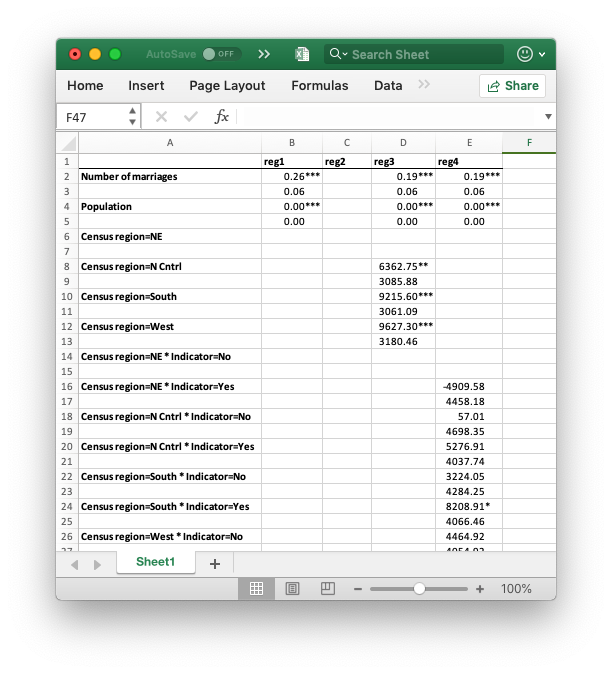
\includegraphics[width=\linewidth]{img/regression}
	\end{figure}
\end{multicols}

\end{frame}


%%%%%%%%%%%%%%%%%%%%%%%%%%%%%%%%%%%%%%%%%%% heading of section 2
\sectionpic{Data Management}{img/section_slide}

\begin{frame}{First Frame}
Content here!
\end{frame}


\begin{frame}{Second Frame}
Content here!
\end{frame}

\begin{frame}[fragile]{Testing Stata code and Text}
\begin{multicols}{2}
	\begin{lstlisting}
	// Data
	sysuse census.dta, clear
	
	// Basic Regression
	reg divorce marriage pop
	est sto reg1
	
	// Basic Regression 2
	reg medage popurban
	est sto reg2
	
	// Indicator Regression
	reg divorce marriage pop i.region
	est sto reg3
	
	// Interaction Regression
	gen binary = rnormal() > 0
	lab def binary 0 "No" 1 "Yes"
	lab val binary binary
	label var binary "Indicator"
	reg divorce marriage pop i.region#i.binary
	est sto reg4
	\end{lstlisting}
	\parbox{\linewidth}{
		This is where you write content describing the Stata code in the text box to the left. Try not to place too much code in the text box. The Stat code is written in the lines before this.
		\newline \newline
		More information about the Stata, giving time for the participants to write the code themselves and run it.
		\newline \newline
		More information about the Stata code and the different ways to code it.
	}
\end{multicols}
\end{frame}

%%%%%%%%%%%%%%%%%%%%%%%%%%%%%%%%%%%%%%%%%%% Final thougts section
\begin{frame}{Conclusion}

Wrap up final contents of presentation

\vspace{20mm}
For more information or further questions please contact:
\newline John Doe (\url{johndoe@worldbank.org}) \newline Mary Doe (\url{marydoe@worldbank.org})

\end{frame}

%%%%%%%%%%%%%%%%%%%%%%%%%%%%%%%%%%%%%%%%%%% The End
\sectionpic{The End}{img/section_slide}






\end{document} 